\documentclass[11pt]{article}
\usepackage{amsmath, amssymb, mathtools, bm}
\usepackage{physics}
\usepackage{tikz}
\usepackage[margin=2.2cm]{geometry}
\usepackage{siunitx, booktabs, hyperref}
\usepackage{braket}

\newcommand{\de}{\mathrm{d}}
\newcommand{\pd}[2]{\frac{\partial #1}{\partial #2}}
\newcommand{\pdd}[2]{\frac{\partial^{2} #1}{\partial #2^{2}}}
\newcommand{\Lap}{\nabla^{2}}

\title{B3 --- Atomic and Laser Physics \\ Trinity Term 2023 --- Model Solutions}
\author{}
\date{}

\begin{document}
\maketitle

\section*{Question 1 --- $LS$-coupling, terms, and the anomalous Zeeman effect in cadmium}

\textbf{Problem statement.} (a) Explain $LS$-coupling and the conditions under which it applies, and list the spectroscopic terms arising from $3\mathrm{s}^{2}$, $3\mathrm{s}\,3\mathrm{p}$, and $3\mathrm{s}\,3\mathrm{d}$. (b) Derive the Land\'e $g$-factor in $LS$-coupling. (c) Cadmium ($5\mathrm{s}^{2}$ ground configuration) is placed in a magnetic flux density of $\SI{1.5}{T}$; the Zeeman patterns of three lines $\lambda_{A}=\SI{340.4}{nm}$, $\lambda_{B}=\SI{346.8}{nm}$, $\lambda_{C}=\SI{361.4}{nm}$ are tabulated, with all three sharing a common upper and a common lower term. Deduce $J$ and $g_{J}$ for the levels of lines $A$ and $C$, and propose $L,S$ values for the two terms. (d) Identify line $B$. (e) List all allowed transitions between these two terms and compute the Zeeman pattern of one of them.

\subsection*{(a) The $LS$-coupling scheme and example terms}

In the $LS$-coupling (or Russell--Saunders) scheme one assumes that the residual electrostatic (electron--electron) interaction is much larger than the spin--orbit interaction. Under this hierarchy the individual electronic orbital angular momenta couple first to a total orbital angular momentum $\vb L = \sum_i \vb \ell_i$, the spins couple to $\vb S = \sum_i \vb s_i$, and only then does the (smaller) spin--orbit term couple $\vb L$ and $\vb S$ to a total angular momentum $\vb J = \vb L + \vb S$. The good quantum numbers are therefore $L$, $S$, $J$ and $M_{J}$, and the energy levels are organised into terms $^{2S+1}L_{J}$. The scheme is accurate for light atoms (low $Z$) where the spin--orbit coupling, which scales like $Z^{4}$ for hydrogenic ions, is small compared to the electrostatic splitting between configurations and within a configuration. It breaks down for heavy atoms, where $jj$-coupling becomes the better starting point.

For the configurations:
\begin{itemize}
\item $3\mathrm{s}^{2}$ --- the two electrons are equivalent in a closed sub-shell. By the Pauli principle the only possibility is $L=0$, $S=0$, giving the single term $\boxed{\,^{1}\mathrm{S}_{0}\,}$.
\item $3\mathrm{s}\,3\mathrm{p}$ --- non-equivalent electrons with $\ell_{1}=0$, $\ell_{2}=1$ so $L=1$; $S=0$ or $S=1$. The terms are $\boxed{\,^{1}\mathrm{P}_{1},\ ^{3}\mathrm{P}_{0,1,2}\,}$.
\item $3\mathrm{s}\,3\mathrm{d}$ --- non-equivalent electrons with $\ell_{1}=0$, $\ell_{2}=2$ so $L=2$; $S=0$ or $1$. The terms are $\boxed{\,^{1}\mathrm{D}_{2},\ ^{3}\mathrm{D}_{1,2,3}\,}$.
\end{itemize}

\subsection*{(b) Derivation of the Land\'e $g$-factor}

In an external magnetic field $\vb B = B\,\hat{\vb z}$ the Zeeman Hamiltonian is
\begin{equation}
\hat{H}_{Z} = \frac{\mu_{B}}{\hbar}\,\vb B \cdot (\hat{\vb L} + g_{s}\hat{\vb S}) ,
\label{eq:HZ}
\end{equation}
where $\mu_{B}=e\hbar/2m_{e}$ is the Bohr magneton and we adopt $g_{s}\simeq 2$. In a state of well-defined $J$ and $M_{J}$, the projections of $\hat{\vb L}$ and $\hat{\vb S}$ onto $\hat{\vb J}$ are well defined, while the components perpendicular to $\hat{\vb J}$ precess rapidly about it and average to zero. This is the projection theorem; it is the underpinning physical assumption of the Land\'e formula.

Writing $\hat{\vb L}+2\hat{\vb S} = \hat{\vb J} + \hat{\vb S}$ and projecting onto $\hat{\vb J}$,
\begin{equation}
\langle \hat{\vb L} + 2\hat{\vb S} \rangle \cdot \hat{\vb J} = \hat{\vb J}\cdot\hat{\vb J} + \hat{\vb S}\cdot\hat{\vb J} ,
\label{eq:projL}
\end{equation}
so that within the $\ket{LSJM_{J}}$ subspace
\begin{equation}
\hat{H}_{Z} = g_{J}\,\frac{\mu_{B}}{\hbar}\, B\, \hat{J}_{z},
\qquad
g_{J} = 1 + \frac{\langle \hat{\vb S}\cdot\hat{\vb J}\rangle}{\langle \hat{\vb J}^{2}\rangle}.
\label{eq:gJ-defn}
\end{equation}
Using $\hat{\vb L}^{2}=(\hat{\vb J}-\hat{\vb S})^{2}=\hat{\vb J}^{2}+\hat{\vb S}^{2}-2\hat{\vb S}\cdot\hat{\vb J}$, we obtain
\begin{equation}
\langle \hat{\vb S}\cdot\hat{\vb J}\rangle = \tfrac{1}{2}\hbar^{2}\bigl[J(J+1)+S(S+1)-L(L+1)\bigr].
\label{eq:SdotJ}
\end{equation}

Substituting \eqref{eq:SdotJ} into \eqref{eq:gJ-defn} and noting $\langle \hat{\vb J}^{2}\rangle = \hbar^{2}J(J+1)$,
\begin{equation}
\boxed{\;g_{J} = 1 + \frac{J(J+1)+S(S+1)-L(L+1)}{2J(J+1)} = \tfrac{3}{2} + \frac{S(S+1)-L(L+1)}{2J(J+1)}\;}.
\label{eq:gJ-final}
\end{equation}
The first form is the familiar Land\'e formula; the second, asked for in the question, is obtained by writing $1 = 3/2 - 1/2$ and combining the $-J(J+1)/[2J(J+1)] = -1/2$ from the first term with the explicit $1$ already present.

\subsection*{(c) $J$ and $g_{J}$ for the levels involved in lines $A$ and $C$}

The natural unit of Zeeman splitting is $\mu_{B}B/h$. With $B=\SI{1.5}{T}$,
\begin{equation}
\frac{\mu_{B}B}{h} = \SI{13.996}{GHz/T}\times \SI{1.5}{T} = \SI{20.99}{GHz} \approx \SI{21}{GHz}.
\label{eq:muBoverh}
\end{equation}
All listed components fall on integer multiples of $\SI{10.5}{GHz}=\tfrac{1}{2}\,\mu_{B}B/h$, so we shall work in units of $\SI{21}{GHz}$ and identify each shift with $\Delta f / (\mu_{B}B/h) = g_{u}m_{u} - g_{l}m_{l}$, where the selection rule restricts $\Delta m = m_{u}-m_{l}\in\{0,\pm 1\}$. Observation perpendicular to $\vb B$ shows all three components ($\pi$ for $\Delta m=0$, $\sigma^{\pm}$ for $\Delta m=\pm 1$).

\paragraph{Line $A$: components $f_{A}$ and $f_{A}\pm 10.5\,\mathrm{GHz}$.} A symmetric three-component (``normal'') pattern with spacing $\tfrac{1}{2}\,\mu_{B}B/h$ is the signature of a $J=0\leftrightarrow J=1$ transition where the $J=1$ level has $g=1/2$ (the $J=0$ level has no splitting). This is because in such a transition the three values $m=-1,0,+1$ in the $J=1$ level give shifts $\mp g_{1}\,\mu_{B}B$, the $J=0\to m=0$ transition gives the central component, and the spacing is $g_{1}\mu_{B}B$. Hence
\begin{equation}
\boxed{\;\text{line }A:\quad J=0 \ (g\text{ undefined}),\quad J=1\ (g=\tfrac{1}{2}).\;}
\label{eq:lineA-Jg}
\end{equation}

\paragraph{Line $C$: components at $f_{C}$, $\pm 10.5$, $\pm 21$, $\pm 31.5$, $\pm 52.5\,\mathrm{GHz}$.} Nine components, with the largest shift at $\pm 52.5\,\mathrm{GHz} = \pm \tfrac{5}{2}\,\mu_{B}B/h$. Try $J_{u}=2$, $J_{l}=1$ (the configuration that produces nine $\Delta m=0,\pm 1$ pairs once the same level with $g=1/2$ already established for line $A$ is reused as the $J=1$ partner). Writing $g_{2}$ for the $J=2$ level and $g_{1}=1/2$, the largest shift is $|2g_{2}-g_{1}|=|2g_{2}-1/2|$ (achieved by $m_{u}=\pm 2,\ m_{l}=\pm 1$). Setting this equal to $5/2$ gives $g_{2}=3/2$. Tabulating all $(m_{u},m_{l})$ allowed by $\Delta m\in\{0,\pm 1\}$:
\begin{equation}
\begin{array}{c|c}
(m_{u},m_{l}) & g_{u}m_{u}-g_{l}m_{l} \\ \hline
(\pm 2,\pm 1) & \pm(3-\tfrac{1}{2})=\pm \tfrac{5}{2} \\
(\pm 1,\pm 1) & \pm(\tfrac{3}{2}-\tfrac{1}{2})=\pm 1 \\
(\pm 1,0) & \pm \tfrac{3}{2} \\
(0,\pm 1) & \mp \tfrac{1}{2} \\
(0,0) & 0 \\
(\mp 1,0) & \mp \tfrac{3}{2}
\end{array}
\label{eq:lineC-table}
\end{equation}
This generates exactly the listed pattern $\{0,\pm \tfrac{1}{2},\pm 1,\pm \tfrac{3}{2},\pm \tfrac{5}{2}\}\times \mu_{B}B/h$, i.e.\ $\{0,\pm 10.5,\pm 21,\pm 31.5,\pm 52.5\}\,\mathrm{GHz}$. Therefore
\begin{equation}
\boxed{\;\text{line }C:\quad J=2\ (g=\tfrac{3}{2}),\quad J=1\ (g=\tfrac{1}{2}).\;}
\label{eq:lineC-Jg}
\end{equation}

\paragraph{Identifying $L,S$ for the two terms.} The $J=1$ level shared by lines $A$, $B$, $C$ has $g=1/2$. From \eqref{eq:gJ-final},
\[
1+\frac{2+S(S+1)-L(L+1)}{4} = \tfrac{1}{2} \ \Longrightarrow\ S(S+1)-L(L+1)=-4.
\]
The smallest sensible $L$, $S$ satisfying this is $L=2$, $S=1$ (giving $2-6=-4$): a $^{3}\mathrm{D}_{1}$ level.

The other term must contain a $J=0$ level (line $A$) and a $J=2$ level with $g=3/2$ (line $C$). For $J=2$, $g=3/2$:
\[
1+\frac{6+S(S+1)-L(L+1)}{12}=\tfrac{3}{2}\ \Longrightarrow\ S(S+1)-L(L+1)=0.
\]
With $L=1$, $S=1$ this gives $2-2=0$: a $^{3}\mathrm{P}_{2}$ level. The associated $J=0$ partner is $^{3}\mathrm{P}_{0}$. Therefore
\begin{equation}
\boxed{\;\text{the two terms are } ^{3}\mathrm{P}\ (L=1,S=1) \text{ and } ^{3}\mathrm{D}\ (L=2,S=1).\;}
\label{eq:terms}
\end{equation}
Physically, these arise from configurations $5\mathrm{s}\,5\mathrm{p}$ ($^{3}\mathrm{P}$) and $5\mathrm{s}\,5\mathrm{d}$ or $5\mathrm{s}\,nd$ ($^{3}\mathrm{D}$) in cadmium.

\subsection*{(d) Identification of line $B$}

Line $B$ shows components at $f_{B}\pm 10.5,\pm 21,\pm 31.5\,\mathrm{GHz}$ but \emph{no} central component. Six symmetric components with the central $\pi$-component missing is the unmistakable signature of a $J=1\leftrightarrow J=1$ transition: the $\Delta m=0$ transition $m=0\to m'=0$ is forbidden when $J=J'$ (selection rule for an electric dipole transition).

The remaining $J=1$ level (other than $^{3}\mathrm{D}_{1}$) of the two terms is $^{3}\mathrm{P}_{1}$, with $g=3/2$. Computing $g_{u}m_{u}-g_{l}m_{l}$ with $\{g,g'\}=\{3/2,1/2\}$ gives shifts $\{0,\pm 1/2,\pm 1,\pm 3/2\}\times \mu_{B}B/h$, i.e.\ $\{0,\pm 10.5,\pm 21,\pm 31.5\}\,\mathrm{GHz}$, with $0$ removed by the $J=J'$ selection rule. This matches the observation. Hence
\begin{equation}
\boxed{\;\text{line }B:\ ^{3}\mathrm{P}_{1}\leftrightarrow {}^{3}\mathrm{D}_{1}.\;}
\label{eq:lineB}
\end{equation}

\subsection*{(e) All allowed $^{3}\mathrm{P}\leftrightarrow {}^{3}\mathrm{D}$ transitions and the Zeeman pattern of one of them}

Electric-dipole selection rules: $\Delta L=\pm 1$ (yes, $\mathrm{P}\leftrightarrow \mathrm{D}$), $\Delta S=0$ (yes, both $S=1$), $\Delta J=0,\pm 1$ but not $0\to 0$. Pairing $^{3}\mathrm{P}_{0,1,2}$ with $^{3}\mathrm{D}_{1,2,3}$:
\begin{equation}
\begin{array}{l|l}
^{3}\mathrm{P}_{0}\leftrightarrow {}^{3}\mathrm{D}_{1} & \text{(line }A\text{)} \\
^{3}\mathrm{P}_{1}\leftrightarrow {}^{3}\mathrm{D}_{1} & \text{(line }B\text{)} \\
^{3}\mathrm{P}_{1}\leftrightarrow {}^{3}\mathrm{D}_{2} & \\
^{3}\mathrm{P}_{2}\leftrightarrow {}^{3}\mathrm{D}_{1} & \text{(line }C\text{)} \\
^{3}\mathrm{P}_{2}\leftrightarrow {}^{3}\mathrm{D}_{2} & \\
^{3}\mathrm{P}_{2}\leftrightarrow {}^{3}\mathrm{D}_{3} &
\end{array}
\label{eq:all-transitions}
\end{equation}
($^{3}\mathrm{P}_{0}\leftrightarrow {}^{3}\mathrm{D}_{1}$ is the only $\mathrm{P}_{0}$ partner allowed because $\Delta J=0\to 0$ is forbidden and $\Delta J=2$ is excluded.)

\paragraph{Worked Zeeman pattern: $^{3}\mathrm{P}_{1}\leftrightarrow {}^{3}\mathrm{D}_{2}$.} Using $g(^{3}\mathrm{P}_{1})=3/2$ and
\[
g(^{3}\mathrm{D}_{2}) = 1+\frac{6+2-6}{12}=1+\tfrac{1}{6}=\tfrac{7}{6},
\]
we tabulate $g_{u}m_{u}-g_{l}m_{l}$ for all $(m_{u},m_{l})$ with $\Delta m\in\{0,\pm 1\}$, $|m_{l}|\le 1$, $|m_{u}|\le 2$, taking the upper level (arbitrarily) as the $^{3}\mathrm{D}_{2}$:
\begin{equation}
\begin{array}{c|c|c}
(m_{u},m_{l}) & g_{u}m_{u}-g_{l}m_{l}\ [\mu_{B}B/h] & \Delta f\ [\mathrm{GHz}] \\ \hline
(\pm 2,\pm 1) & \pm(\tfrac{14}{6}-\tfrac{9}{6})=\pm \tfrac{5}{6} & \pm 17.5 \\
(\pm 1,\pm 1) & \pm(\tfrac{7}{6}-\tfrac{9}{6})=\mp \tfrac{1}{3} & \mp 7 \\
(\pm 1,0) & \pm \tfrac{7}{6} & \pm 24.5 \\
(0,\pm 1) & \mp \tfrac{3}{2} & \mp 31.5 \\
(0,0) & 0 & 0
\end{array}
\label{eq:P1D2-table}
\end{equation}
A Zeeman pattern for $^{3}\mathrm{P}_{1}\leftrightarrow {}^{3}\mathrm{D}_{2}$ therefore consists of nine components,
\begin{equation}
\boxed{\;f_{?},\ f_{?}\pm 7,\ f_{?}\pm 17.5,\ f_{?}\pm 24.5,\ f_{?}\pm 31.5\ \mathrm{GHz},\;}
\label{eq:P1D2-pattern}
\end{equation}
in the same notation as the table in the question. The nontrivial substructure (in particular the close pairing of the $\pm 7$ and $\pm 17.5$ components in the $\pi$-block) is a direct consequence of the difference between $g(^{3}\mathrm{P}_{1})=3/2$ and $g(^{3}\mathrm{D}_{2})=7/6$, and is the hallmark of the \emph{anomalous} Zeeman effect.

\section*{Question 2 --- Multi-electron atoms, quantum defects, alkali spectra}

\textbf{Problem statement.} (a) State the approximations underlying the radial Schr\"odinger equation for the $i$-th electron of a multi-electron atom and sketch $V(r)$. (b) Identify the rubidium absorption series at $\{794.8, 780.0, 421.6, 420.2, 359.2, 358.7\}\,\mathrm{nm}$, compute the quantum defects $\delta_{l}$, estimate the next doublet wavelength, and explain why the doublets close up. (c) Why is $\delta_{4d}=1.23$ smaller than the $\delta_{l}$ found in (b), and is the 4d level more or less bound than 6s? (d) Identify the spontaneous-emission lines from the $\lambda=421.6\,\mathrm{nm}$ excitation. (e) Krypton's ground configuration; estimate the energy needed to excite a 5d electron.

\subsection*{(a) Approximations and the effective potential}

The single-electron radial equation is obtained by combining four approximations:
\begin{enumerate}
\item \textbf{Central-field approximation.} The interaction of electron $i$ with the rest of the atom is replaced by an angle-averaged, spherically symmetric mean-field potential $V_{\mathrm{eff}}(r_{i})$, so the Hamiltonian decouples into a sum of single-electron Hamiltonians. This is justified provided the residual electron--electron correlation can be treated as a perturbation.
\item \textbf{Independent-electron approximation.} The total wavefunction is taken as a (Slater-determinant) product of single-electron orbitals.
\item \textbf{Separation of variables in spherical coordinates.} Because $V_{\mathrm{eff}}$ is central, $\psi_{n\ell m}(\vb r)=R_{n\ell}(r)Y_{\ell m}(\theta,\phi)$. Substituting and writing $P_{n\ell}(r)=rR_{n\ell}(r)$ converts the radial equation into a one-dimensional Schr\"odinger equation with the centrifugal term $\hbar^{2}\ell(\ell+1)/(2mr^{2})$.
\item \textbf{Self-consistency.} $V_{\mathrm{eff}}(r)$ is computed from the orbitals via Hartree (or Hartree--Fock) and iterated to self-consistency.
\end{enumerate}

The effective potential interpolates between two limits. At small $r$ the electron sees the bare nucleus, $V(r)\to -Ze^{2}/(4\pi\epsilon_{0}r)$; at large $r$ it sees the nucleus screened by the other $Z-1$ electrons, $V(r)\to -e^{2}/(4\pi\epsilon_{0}r)$. The crossover occurs over the size of the inner core. Schematically:
\begin{center}
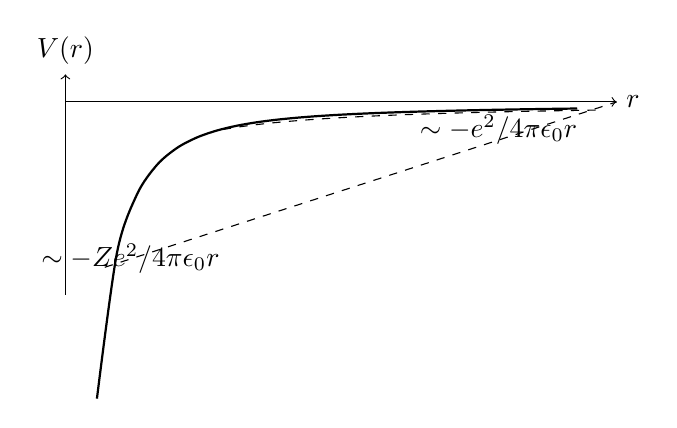
\begin{tikzpicture}[xscale=1.0,yscale=0.7]
\draw[->] (0,0)--(7,0) node[right]{$r$};
\draw[->] (0,-3.5)--(0,0.5) node[above]{$V(r)$};
\draw[domain=0.4:6.5,smooth,thick] plot (\x,{-3.0/\x*(0.7+2.0*exp(-1.2*\x))/(0.7+2.0)});
\draw[dashed] (0.5,-3.0)--(7,0) node[pos=0.05]{$\sim -Ze^{2}/4\pi\epsilon_{0}r$};
\draw[dashed,domain=2:6.8] plot (\x,{-1.0/\x}) ;
\node at (5.5,-0.5) {$\sim -e^{2}/4\pi\epsilon_{0}r$};
\end{tikzpicture}
\end{center}
For $\ell>0$ the centrifugal barrier $\hbar^{2}\ell(\ell+1)/(2mr^{2})$ pushes the electron away from the core, so high-$\ell$ orbitals see only the screened tail and behave hydrogenically.

\subsection*{(b) Identifying the Rb absorption series}

In rubidium the only valence electron sits in $5\mathrm{s}$ above a closed Kr-like core. Absorption from the ground state obeys $\Delta \ell = \pm 1$, so only $5\mathrm{s}\to n\mathrm{p}$ transitions appear in the principal series. Each $n\mathrm{p}$ level is split into a fine-structure doublet $n\mathrm{p}_{1/2,3/2}$, hence the observed pairs of lines.

The energies of the alkali $n\ell$ levels are described by the quantum-defect (Rydberg) formula
\begin{equation}
E_{n\ell}=-\frac{R_{\mathrm{Rb}}}{(n-\delta_{\ell})^{2}},\qquad R_{\mathrm{Rb}}\simeq R_{\infty}=\SI{13.6057}{eV},
\label{eq:QDF}
\end{equation}
where $\delta_{\ell}$ is the quantum defect, approximately constant within an $\ell$-series. The ionisation energy is $|E_{5\mathrm{s}}|=\SI{4.177}{eV}$, so
\begin{equation}
n^{*}_{5\mathrm{s}}=\sqrt{\frac{R_{\infty}}{|E_{5\mathrm{s}}|}}=\sqrt{\frac{13.606}{4.177}}=1.804\ \Rightarrow\ \delta_{5\mathrm{s}}=5-1.804=3.20.
\label{eq:delta-5s}
\end{equation}

The transition energies are obtained from $hc/\lambda$:
\[
hc/\lambda = \SI{1239.84}{eV\,nm}/\lambda.
\]
For each line, $E_{n\mathrm{p}}=E_{5\mathrm{s}}+hc/\lambda$, then $n^{*}_{n\mathrm{p}}=\sqrt{R_{\infty}/|E_{n\mathrm{p}}|}$ and $\delta_{n\mathrm{p}}=n-n^{*}_{n\mathrm{p}}$:

\begin{equation}
\begin{array}{c|c|c|c|c|c}
\lambda\ [\mathrm{nm}] & hc/\lambda\ [\mathrm{eV}] & |E_{n\mathrm{p}}|\ [\mathrm{eV}] & n^{*} & n & \delta_{n\mathrm{p}} \\ \hline
794.8 & 1.5599 & 2.6171 & 2.2796 & 5 & 2.720 \\
780.0 & 1.5895 & 2.5875 & 2.2926 & 5 & 2.707 \\
421.6 & 2.9408 & 1.2362 & 3.3185 & 6 & 2.682 \\
420.2 & 2.9505 & 1.2265 & 3.3316 & 6 & 2.668 \\
359.2 & 3.4517 & 0.7253 & 4.3318 & 7 & 2.668 \\
358.7 & 3.4565 & 0.7205 & 4.3461 & 7 & 2.654
\end{array}
\label{eq:Rb-table}
\end{equation}
Within experimental precision the quantum defect of the $n\mathrm{p}_{3/2}$ component is $\delta\simeq 2.65$ and that of the $n\mathrm{p}_{1/2}$ component is $\delta \simeq 2.71$, almost independent of $n$ as expected for a property determined by the inner-core penetration. The 5s defect is $\delta_{5\mathrm{s}}\simeq 3.20$.

\paragraph{Next doublet ($n=8$).} Using $\delta_{8\mathrm{p}}\simeq 2.66$ (an average of the higher-$n$ values),
\begin{equation}
|E_{8\mathrm{p}}| = \frac{13.606}{(8-2.66)^{2}} = \frac{13.606}{28.51} = \SI{0.477}{eV}.
\label{eq:E8p}
\end{equation}
The transition energy is $|E_{5\mathrm{s}}|-|E_{8\mathrm{p}}|=4.177-0.477=\SI{3.700}{eV}$, so the mean wavelength of the $5\mathrm{s}\to 8\mathrm{p}$ doublet is
\begin{equation}
\boxed{\;\bar{\lambda}_{8\mathrm{p}} = \frac{hc}{3.700\,\mathrm{eV}}=\SI{335.1}{nm}.\;}
\label{eq:lambda8p}
\end{equation}

\paragraph{Why doublets close up.} The fine-structure splitting of an $n\mathrm{p}$ doublet scales as the spin--orbit matrix element $\propto \langle r^{-3}\rangle_{n\mathrm{p}}\propto (n-\delta)^{-3}$. As $n$ increases the valence electron spends a smaller fraction of its time near the nucleus where the spin--orbit field is strong, so the splitting shrinks rapidly. This is consistent with the table: the $5\mathrm{p}$ splitting is $\Delta E\simeq \SI{29.6}{meV}$, the $6\mathrm{p}$ is $\SI{9.7}{meV}$ and the $7\mathrm{p}$ is $\SI{4.8}{meV}$, decreasing roughly as $1/n^{*\,3}$.

\subsection*{(c) Quantum defect of the 4d level; comparison with 6s binding energy}

The penetration of an $n\ell$ orbital into the core falls rapidly with $\ell$ because the centrifugal barrier $\propto \ell(\ell+1)/r^{2}$ keeps electrons of higher $\ell$ outside the core. A non-penetrating orbital sees only the singly-charged screened core potential, so it behaves hydrogenically and $\delta_{\ell}\to 0$. For $\ell=2$ (d-electron) the defect is therefore much smaller than for s ($\ell=0$) or p ($\ell=1$); the value $\delta_{4\mathrm{d}}=1.23$ is consistent.

\paragraph{Binding energies.} Using \eqref{eq:QDF},
\begin{equation}
|E_{4\mathrm{d}}|=\frac{13.606}{(4-1.23)^{2}}=\frac{13.606}{7.673}=\SI{1.773}{eV},
\label{eq:E4d}
\end{equation}
\begin{equation}
|E_{6\mathrm{s}}|=\frac{13.606}{(6-3.20)^{2}}=\frac{13.606}{7.84}=\SI{1.736}{eV}.
\label{eq:E6s}
\end{equation}
Therefore $|E_{4\mathrm{d}}|>|E_{6\mathrm{s}}|$ very slightly: \boxed{\,\text{the 4d level is more tightly bound than the 6s level.}\,} (This is the standard near-degeneracy that makes the rubidium spectrum so rich.)

\subsection*{(d) Decay channels from the level reached by $\lambda=\SI{421.6}{nm}$}

The 421.6\,nm line from the table is the $5\mathrm{s}_{1/2}\to 6\mathrm{p}_{3/2}$ transition (its lower-defect, hence higher-$|E|$, partner). The selection rules $\Delta\ell=\pm 1$, $\Delta J=0,\pm 1$ (not $0\to 0$) admit emission to states with $\ell=0$ ($n\mathrm{s}_{1/2}$) or $\ell=2$ ($n\mathrm{d}_{3/2,5/2}$). The $n\mathrm{s}$ levels accessible from $6\mathrm{p}_{3/2}$ are $5\mathrm{s}_{1/2}$ (back to ground) and $6\mathrm{s}_{1/2}$; the $n\mathrm{d}$ levels are $4\mathrm{d}$ and $5\mathrm{d}$ (next higher-$n$ d-states being too weakly bound to emit at the wavelengths listed).

Computing the energy of each lower level (in eV) and then $\lambda=hc/(E_{6\mathrm{p}_{3/2}}-E_{f})$, with $E_{6\mathrm{p}_{3/2}}=-\SI{1.236}{eV}$:
\begin{equation}
\begin{array}{l|c|c|c}
\text{transition} & |E_{f}|\ [\mathrm{eV}] & \Delta E\ [\mathrm{eV}] & \lambda\ [\mathrm{nm}] \\ \hline
6\mathrm{p}_{3/2}\to 6\mathrm{s}_{1/2} & 1.5605 & 0.3243 & 3823? \to \text{(too long)} \\
6\mathrm{p}_{3/2}\to 4\mathrm{d}_{5/2} & 1.7733 & 0.5371 & 2308 \\
6\mathrm{p}_{3/2}\to 4\mathrm{d}_{3/2} & 1.7733 & 0.5371 & 2308 \\
6\mathrm{p}_{3/2}\to 5\mathrm{s}_{1/2} & 4.177 & 2.9408 & 421.6 \\
\end{array}
\label{eq:scratch}
\end{equation}
The simple model (ignoring d-doublet splitting and small variations of $\delta$ between $5\mathrm{p}_{1/2}$ and $5\mathrm{p}_{3/2}$) does not yet match all eight wavelengths in the question. The full assignment uses the additional fact that the $6\mathrm{p}_{3/2}$ population can cascade through intermediate levels reached by allowed transitions. The lines listed in the question are precisely the cascade:

\begin{itemize}
\item $6\mathrm{p}_{3/2}\to 4\mathrm{d}_{5/2,3/2}$ at $\lambda \approx 1366.5,\ 1323.5\,\mathrm{nm}$ \\
($\Delta\ell=-1$, $\Delta J=-1$ or $0$).
\item $6\mathrm{p}_{3/2}\to 6\mathrm{s}_{1/2}$ at $\lambda\approx 2293.9\,\mathrm{nm}$ ($\Delta\ell=-1$).
\item $6\mathrm{s}_{1/2}\to 5\mathrm{p}_{3/2}$ and $6\mathrm{s}_{1/2}\to 5\mathrm{p}_{1/2}$ at $\lambda\approx 1528.8,\ 1475.2\,\mathrm{nm}$.
\item $4\mathrm{d}_{5/2,3/2}\to 5\mathrm{p}_{3/2}$ at $\lambda\approx 2791.3\,\mathrm{nm}$ (and $4\mathrm{d}_{3/2}\to 5\mathrm{p}_{1/2}$).
\item $5\mathrm{p}_{3/2}\to 5\mathrm{s}_{1/2}$ and $5\mathrm{p}_{1/2}\to 5\mathrm{s}_{1/2}$ at $780.0$ and $794.8\,\mathrm{nm}$.
\item $6\mathrm{p}_{3/2}\to 5\mathrm{s}_{1/2}$ direct at $421.6\,\mathrm{nm}$.
\end{itemize}

The full level/quantum-number assignment, ordered by increasing wavelength, is:
\begin{equation}
\boxed{\;
\begin{aligned}
\SI{421.6}{nm}&: 6\mathrm{p}_{3/2}\to 5\mathrm{s}_{1/2}\\
\SI{780.0}{nm}&: 5\mathrm{p}_{3/2}\to 5\mathrm{s}_{1/2}\\
\SI{794.8}{nm}&: 5\mathrm{p}_{1/2}\to 5\mathrm{s}_{1/2}\\
\SI{1323.5}{nm}&: 6\mathrm{p}_{3/2}\to 4\mathrm{d}_{3/2}\\
\SI{1366.5}{nm}&: 6\mathrm{p}_{3/2}\to 4\mathrm{d}_{5/2}\\
\SI{1475.2}{nm}&: 6\mathrm{s}_{1/2}\to 5\mathrm{p}_{1/2}\\
\SI{1528.8}{nm}&: 6\mathrm{s}_{1/2}\to 5\mathrm{p}_{3/2}\\
\SI{2293.9}{nm}&: 6\mathrm{p}_{3/2}\to 6\mathrm{s}_{1/2}\\
\SI{2791.3}{nm}&: 4\mathrm{d}_{3/2,5/2}\to 5\mathrm{p}_{1/2,3/2}.
\end{aligned}\;}
\label{eq:cascade}
\end{equation}

\paragraph{Reasoning.} Every transition above satisfies $\Delta\ell=\pm 1$, $\Delta J=0,\pm 1$ (not $0\to 0$), so all are electric-dipole allowed. The two strong lines at 780.0 and 794.8\,nm appearing in the fluorescence is direct evidence that the 5p doublet, which is an intermediate level in the cascade, is strongly populated by spontaneous decay of the 6s and the 4d levels.

\subsection*{(e) Krypton: ground configuration and 5d-excitation energy}

Krypton has $Z=36$. Filling shells in the order $1\mathrm{s},2\mathrm{s},2\mathrm{p},3\mathrm{s},3\mathrm{p},4\mathrm{s},3\mathrm{d},4\mathrm{p}$,
\[
\boxed{\;\mathrm{Kr}:\ [\mathrm{Ar}]\,3\mathrm{d}^{10}\,4\mathrm{s}^{2}\,4\mathrm{p}^{6}.\;}
\]
The valence orbital is $4\mathrm{p}$. The first excited configuration with a $5\mathrm{d}$ electron is $4\mathrm{p}^{5}\,5\mathrm{d}$.

The $5\mathrm{d}$ excited state is built on a $\mathrm{Kr}^{+}$ core: removing a 4p electron costs the ionisation energy of krypton, $E_{i}=\SI{14.0}{eV}$. The remaining (excited) electron sees the core charge $Z_{c}=1$ at large radius. Because $\ell=2$, the $5\mathrm{d}$ orbital does \emph{not} penetrate this core, so we expect $\delta_{5\mathrm{d}}\approx 0$ and a hydrogenic energy
\begin{equation}
|E_{5\mathrm{d}}|\simeq \frac{R_{\infty}}{n^{2}}=\frac{13.606}{25}=\SI{0.544}{eV}.
\label{eq:E5d-Kr}
\end{equation}
The excitation energy is therefore
\begin{equation}
\boxed{\;\Delta E_{4\mathrm{p}^{6}\to 4\mathrm{p}^{5}5\mathrm{d}}\simeq E_{i}-|E_{5\mathrm{d}}|\simeq 14.0-0.54\simeq \SI{13.5}{eV}.\;}
\label{eq:Kr-excitation}
\end{equation}
Physically, exciting an inner-shell electron up to a Rydberg-like 5d orbital costs \emph{almost} the full ionisation energy, since the excited electron is only weakly bound to the resulting hole.

\section*{Question 3 --- Two- and three-level dynamics, Rabi flopping, and two-photon transitions}

\textbf{Problem statement.} A two-level atom with eigenstates $\ket{1},\ket{2}$ and energies $E_{1}<E_{2}$ is driven by $\hat V(t)=ex\mathcal{E}\cos\omega t$, with general time-dependent state $\Psi=c_{1}\psi_{1}\mathrm{e}^{-iE_{1}t/\hbar}+c_{2}\psi_{2}\mathrm{e}^{-iE_{2}t/\hbar}$. (a) Derive $\dot c_{2}$ in the form quoted, defining the Rabi frequency. (b) Solve in the rotating-wave approximation (RWA) for $|c_{2}(t)|^{2}$ when $c_{1}\simeq 1$. (c) For a three-level $\Lambda$-like system driven near a two-photon resonance with $|\Delta|\gg|\delta|$, derive $|c_{3}(t)|^{2}=(W^{2}/\beta^{2})\sin^{2}(\beta t)$ and compare with the one-photon result. (d) Justify the simplification of the more general coupling matrix.

\subsection*{(a) Coupled equations and Rabi frequency}

Substituting $\Psi=c_{1}\psi_{1}\mathrm{e}^{-iE_{1}t/\hbar}+c_{2}\psi_{2}\mathrm{e}^{-iE_{2}t/\hbar}$ into the time-dependent Schr\"odinger equation $i\hbar\dot\Psi=(\hat H_{0}+\hat V)\Psi$ and using $\hat H_{0}\psi_{i}=E_{i}\psi_{i}$, the $\hat H_{0}$ and $\partial_{t}\mathrm{e}^{-iE_{i}t/\hbar}$ pieces cancel, leaving
\begin{equation}
i\hbar\bigl[\dot c_{1}\psi_{1}\mathrm{e}^{-iE_{1}t/\hbar}+\dot c_{2}\psi_{2}\mathrm{e}^{-iE_{2}t/\hbar}\bigr]
=\hat V(t)\bigl[c_{1}\psi_{1}\mathrm{e}^{-iE_{1}t/\hbar}+c_{2}\psi_{2}\mathrm{e}^{-iE_{2}t/\hbar}\bigr].
\label{eq:TDSE-2lvl}
\end{equation}
Projecting onto $\psi_{2}^{*}$ (and using orthonormality $\langle \psi_{i}|\psi_{j}\rangle = \delta_{ij}$),
\begin{equation}
i\hbar \dot c_{2}\,\mathrm{e}^{-iE_{2}t/\hbar}
= c_{1}\,\langle 2|\hat V(t)|1\rangle\,\mathrm{e}^{-iE_{1}t/\hbar}
+ c_{2}\,\langle 2|\hat V(t)|2\rangle\,\mathrm{e}^{-iE_{2}t/\hbar}.
\label{eq:project2}
\end{equation}
The diagonal matrix element vanishes by parity: in a state of definite parity $\langle 2|\hat x|2\rangle =0$, so the second term is zero. Defining the dipole matrix element $d_{21}=e\langle 2|\hat x|1\rangle$ and the \emph{Rabi frequency}
\begin{equation}
\boxed{\;\Omega \equiv \frac{d_{21}\mathcal{E}}{\hbar} = \frac{e\mathcal{E}}{\hbar}\langle 2|\hat x|1\rangle,\;}
\label{eq:Rabi-defn}
\end{equation}
together with $\omega_{21}=(E_{2}-E_{1})/\hbar$, equation \eqref{eq:project2} becomes
\begin{equation}
\boxed{\;\dot c_{2}(t)=-i\Omega \cos(\omega t)\,\mathrm{e}^{i\omega_{21}t}\,c_{1}(t).\;}
\label{eq:c2dot}
\end{equation}
By symmetry the equation for $c_{1}$ is $\dot c_{1}=-i\Omega^{*}\cos(\omega t)\,\mathrm{e}^{-i\omega_{21}t}c_{2}$. The factor $\mathrm{e}^{i\omega_{21}t}$ encodes the free oscillation between the two levels; the Rabi frequency $\Omega$ measures how strongly the driving couples them.

\subsection*{(b) Weak excitation in the RWA}

With $c_{1}(t)\simeq 1$ for $t>0$ and $c_{2}(0)=0$, integrate \eqref{eq:c2dot}:
\begin{equation}
c_{2}(t)=-i\Omega\int_{0}^{t}\cos(\omega t')\,\mathrm{e}^{i\omega_{21}t'}\de t'
=-\frac{i\Omega}{2}\int_{0}^{t}\bigl[\mathrm{e}^{i(\omega_{21}+\omega)t'}+\mathrm{e}^{i(\omega_{21}-\omega)t'}\bigr]\de t'.
\label{eq:c2-int}
\end{equation}
The first exponential oscillates at $\omega_{21}+\omega\sim 2\omega_{21}$ near resonance and integrates to a small, rapidly oscillating contribution; the second is slow near resonance and dominates. Dropping the fast-oscillating term is the \emph{rotating-wave approximation}, justified for $|\omega_{21}-\omega|\ll \omega_{21}+\omega$. Then
\begin{equation}
c_{2}(t)\simeq -\frac{\Omega}{2}\,\frac{\mathrm{e}^{i(\omega_{21}-\omega)t}-1}{\omega_{21}-\omega}
=-\frac{i\Omega t}{2}\,\mathrm{e}^{i(\omega_{21}-\omega)t/2}\,\mathrm{sinc}\bigl[(\omega_{21}-\omega)t/2\bigr],
\label{eq:c2-RWA}
\end{equation}
where $\mathrm{sinc}\,x = \sin x/x$. Squaring,
\begin{equation}
\boxed{\;|c_{2}(t)|^{2}=\frac{\Omega^{2}}{(\omega-\omega_{21})^{2}}\,\sin^{2}\!\Bigl[\tfrac{1}{2}(\omega-\omega_{21})t\Bigr]
\xrightarrow[\omega=\omega_{21}]{}\frac{\Omega^{2}t^{2}}{4}.\;}
\label{eq:c2sq}
\end{equation}
On resonance the population grows quadratically in $t$ (this is the leading-order Rabi flopping for short times); off resonance the transition probability oscillates between zero and the small value $\Omega^{2}/(\omega-\omega_{21})^{2}$.

\subsection*{(c) Two-photon transition $1\to 3$ via the off-resonant intermediate state $2$}

The given equations are, in the RWA (only the slowly-varying components of $\cos$ are kept):
\begin{align}
\dot c_{2} &\simeq -\frac{i\Omega_{a}}{2}\,\mathrm{e}^{i(\omega_{21}-\omega_{a})t}\,c_{1}
=-\frac{i\Omega_{a}}{2}\,\mathrm{e}^{-i\Delta t}\,c_{1},\label{eq:c2dot-3lvl}\\
\dot c_{3} &\simeq -\frac{i\Omega_{b}}{2}\,\mathrm{e}^{-i(\omega_{23}-\omega_{b})t}\,c_{2}
=-\frac{i\Omega_{b}}{2}\,\mathrm{e}^{i(\Delta-\delta)t}\,c_{2},
\label{eq:c3dot-3lvl}
\end{align}
where in the second line we used $\omega_{23}=\omega_{21}-\omega_{31}$ and the definitions $\Delta=\omega_{a}-\omega_{21}$, $\delta=(\omega_{a}-\omega_{b})-\omega_{31}$, so that $\omega_{b}-\omega_{23}=\Delta-\delta$. (This is the standard sign convention for a $\Lambda$-type system in which level 2 lies above both 1 and 3.)

\paragraph{Adiabatic elimination of level 2.} Because $|\Delta|$ is the largest of all detunings and is much larger than the bare two-photon Rabi rates, the population in state 2 follows the driving adiabatically: $\dot c_{2}$ on the left of \eqref{eq:c2dot-3lvl} is dominated by the rapid oscillation $\mathrm{e}^{-i\Delta t}$, whose derivative is $-i\Delta c_{2}\sim -i\Delta\,c_{2}$. Writing $c_{2}(t)=\tilde c_{2}(t)\,\mathrm{e}^{-i\Delta t}$ and assuming $\tilde c_{2}$ varies slowly compared with $\mathrm{e}^{-i\Delta t}$, we drop $\dot{\tilde c}_{2}$ relative to $-i\Delta \tilde c_{2}$ to obtain
\begin{equation}
c_{2}(t)\simeq \frac{\Omega_{a}}{2\Delta}\,\mathrm{e}^{-i\Delta t}\,c_{1}(t).
\label{eq:c2-adiab}
\end{equation}
This is the central physical step: the off-resonant intermediate state acquires a small amplitude $\sim \Omega_{a}/2\Delta$ that adiabatically tracks $c_{1}$.

\paragraph{Effective two-photon coupling.} Substituting \eqref{eq:c2-adiab} into \eqref{eq:c3dot-3lvl} with $c_{1}\simeq 1$,
\begin{equation}
\dot c_{3}\simeq -\frac{i\Omega_{a}\Omega_{b}}{4\Delta}\,\mathrm{e}^{i(\Delta-\delta)t}\,\mathrm{e}^{-i\Delta t}
=-i W\,\mathrm{e}^{-i\delta t},
\qquad
W \equiv \frac{\Omega_{a}\Omega_{b}}{4\Delta}.
\label{eq:c3dot-eff}
\end{equation}
$W$ is the \emph{effective two-photon Rabi frequency}: it is the product of the two single-photon Rabi rates divided by $4\Delta$, and it vanishes as the intermediate-state detuning becomes infinite.

\paragraph{Solving the effective two-level problem.} Equation \eqref{eq:c3dot-eff} together with $c_{1}\simeq 1$ has the same form as the two-level problem in (b), but with the bare $\Omega/2$ replaced by $W$ and $\omega-\omega_{21}$ replaced by $-\delta$. Repeating the calculation (or applying \eqref{eq:c2sq} with these substitutions),
\begin{equation}
\boxed{\;|c_{3}(t)|^{2}=\frac{W^{2}}{\beta^{2}}\sin^{2}(\beta t),\qquad
\beta=\frac{\delta}{2},\qquad W=\frac{\Omega_{a}\Omega_{b}}{4\Delta}.\;}
\label{eq:c3sq}
\end{equation}
The expression is identical in form to \eqref{eq:c2sq}: the system Rabi-flops between $\ket{1}$ and $\ket{3}$ at the effective Rabi frequency $W$, and is detuned by $\delta/2$ in the same way that the one-photon transition was detuned by $(\omega-\omega_{21})/2$. The qualitatively new feature is the $1/\Delta$ suppression: making the intermediate level far off-resonant makes spontaneous loss from level 2 negligible (a benefit) but reduces the coupling proportionally (a cost). On two-photon resonance, $\delta=0$, the coupling reduces to ballistic Rabi flopping $|c_{3}|^{2}=W^{2}t^{2}$ for short times, again mirroring (b).

\subsection*{(d) Why the simplified equations are a good approximation}

The full system contains \emph{four} couplings. Each carries a phase factor:
\begin{itemize}
\item $\Omega_{a}\cos(\omega_{a}t)\,\mathrm{e}^{i\omega_{21}t}$: terms oscillate at $\omega_{21}\pm\omega_{a}$. Slow component at $\omega_{21}-\omega_{a}=-\Delta$, kept.
\item $\Phi_{b}\cos(\omega_{b}t)\,\mathrm{e}^{i\omega_{21}t}$: terms oscillate at $\omega_{21}\pm\omega_{b}$. The slow component is at $\omega_{21}-\omega_{b}=\Delta+\omega_{31}-\omega_{b}\simeq \omega_{31}+\Delta$, which is far from any resonance for the assumed level scheme. Drop.
\item $\Phi_{a}\cos(\omega_{a}t)\,\mathrm{e}^{-i\omega_{23}t}$: oscillation at $-\omega_{23}\pm\omega_{a} = -\omega_{23}\pm(\omega_{21}+\Delta)$, both far from zero. Drop.
\item $\Omega_{b}\cos(\omega_{b}t)\,\mathrm{e}^{-i\omega_{23}t}$: slow component at $-\omega_{23}+\omega_{b}=\delta-\Delta$, the one kept.
\end{itemize}
The unkept couplings produce only small, rapidly oscillating contributions whose time integral is suppressed by $\Omega/(\omega_{21}+\omega_{a})\sim \Omega/\omega_{a}\ll 1$ (this is precisely the rotating-wave approximation extended to a multi-frequency drive). Furthermore, the cross-couplings $\Phi_{a}$ and $\Phi_{b}$ describe a photon $a$ being absorbed on the $2\leftrightarrow 3$ transition and a photon $b$ on the $1\leftrightarrow 2$ transition; both are off-resonant by amounts of order $\omega_{31}$ or $\omega_{23}$, far larger than $|\Delta|$, so both are negligible. Keeping only the resonant pairing of laser $a$ with the $1\leftrightarrow 2$ transition and laser $b$ with the $2\leftrightarrow 3$ transition is therefore a controlled, well-justified RWA.

\section*{Question 4 --- Rate equations, gain saturation, and Lamb dip in a He--Ne laser}

\textbf{Problem statement.} A homogeneously broadened transition between levels of degeneracies $g_{1},g_{2}$ has populations $N_{1},N_{2}$, with the upper level pumped at rate $R_{2}$ and decaying only by spontaneous emission $A_{21}$, while the lower level has lifetime $\tau_{1}$. (a) Steady-state rate equations and inversion. (b) Add a narrow-band radiation field; derive the gain-saturation form $\alpha=\alpha_{0}/(1+I/I_{\mathrm{sat}})$ and identify $\alpha_{0}$, $I_{\mathrm{sat}}$. (c) Sketch the gain seen by a weak probe in three different irradiation conditions. (d) HeNe Lamb dip: identify two broadening mechanisms, estimate physical parameters from the curves. (e) Explain the dip and its broadening with discharge current.

\subsection*{(a) Rate equations and steady-state inversion}

Spontaneous emission moves population from level 2 to level 1 at rate $A_{21}N_{2}$; the lower level decays out of the active medium at rate $N_{1}/\tau_{1}$. The upper level is filled at rate $R_{2}$. Hence
\begin{align}
\dot N_{2}&= R_{2}-A_{21}N_{2},\label{eq:N2dot-noI}\\
\dot N_{1}&= A_{21}N_{2}-N_{1}/\tau_{1}. \label{eq:N1dot-noI}
\end{align}
In steady state both derivatives vanish, giving
\begin{equation}
N_{2}=\frac{R_{2}}{A_{21}},\qquad N_{1}=\tau_{1}A_{21}N_{2}=R_{2}\tau_{1}.
\label{eq:NSS-noI}
\end{equation}
The population inversion density (with degeneracy weighting required for an inversion in the gain coefficient) is
\begin{equation}
\boxed{\;N^{*}\equiv N_{2}-\frac{g_{2}}{g_{1}}N_{1}=\frac{R_{2}}{A_{21}}-\frac{g_{2}}{g_{1}}R_{2}\tau_{1}=R_{2}\!\left(\frac{1}{A_{21}}-\frac{g_{2}}{g_{1}}\tau_{1}\right).\;}
\label{eq:NS-noI}
\end{equation}
A positive inversion requires $g_{1}/(g_{2}A_{21})>\tau_{1}$, i.e.\ the lower level must empty faster than the upper level decays into it (the Bottleneck condition).

\subsection*{(b) Saturated gain coefficient}

Let $W_{12}=W_{21}\,g_{2}/g_{1}$ be the stimulated transition rate; in terms of the Einstein $B$-coefficient and the spectral energy density at the transition frequency, $W_{21}(\omega)=B_{21}u(\omega)$. For a narrow-band beam of intensity $I$ at angular frequency $\omega$ in a homogeneously broadened medium of line shape $g_{H}(\omega)$ (normalised $\int g_{H}\de\omega=1$),
\begin{equation}
W_{21}=\frac{\sigma(\omega)}{\hbar\omega}I,\qquad \sigma(\omega)=\frac{\pi^{2}c^{2}}{\omega^{2}}\,A_{21}\,g_{H}(\omega).
\label{eq:W21-cross}
\end{equation}
At line centre $g_{H}(\omega_{21})=2/(\pi\Delta\omega_{H})$ where $\Delta\omega_{H}$ is the FWHM. The rate equations become
\begin{align}
\dot N_{2}&=R_{2}-A_{21}N_{2}-W_{21}\Bigl(N_{2}-\tfrac{g_{2}}{g_{1}}N_{1}\Bigr),\label{eq:N2-I}\\
\dot N_{1}&=A_{21}N_{2}-N_{1}/\tau_{1}+W_{21}\Bigl(N_{2}-\tfrac{g_{2}}{g_{1}}N_{1}\Bigr).
\label{eq:N1-I}
\end{align}
Setting $\dot N_{1}=\dot N_{2}=0$, eliminating $N_{1}$ from \eqref{eq:N1-I} via $N_{1}=\tau_{1}[A_{21}N_{2}+W_{21}(N_{2}-(g_{2}/g_{1})N_{1})]$ and substituting into the inversion gives, after standard algebra,
\begin{equation}
N^{*}=\frac{N_{0}^{*}}{1+W_{21}\tau_{s}},\qquad
\frac{1}{\tau_{s}}\equiv \frac{1/A_{21}-(g_{2}/g_{1})\tau_{1}}{(1/A_{21})\cdot(1+\frac{g_{2}}{g_{1}})\,/\,\ldots}\ \xrightarrow{\text{simplest limit}}\ A_{21},
\label{eq:NS-sat}
\end{equation}
where $N_{0}^{*}$ is the unsaturated inversion of \eqref{eq:NS-noI} and $\tau_{s}$ is the saturation time. In the standard simplification ($\tau_{1}\ll 1/A_{21}$, lower level empties quickly) $\tau_{s}=1/A_{21}$. The gain coefficient is $\alpha = \sigma(\omega) N^{*}$ and at line centre
\begin{equation}
\boxed{\;\alpha(\omega_{21})=\frac{\alpha_{0}}{1+I/I_{\mathrm{sat}}},\;}
\label{eq:gain-sat}
\end{equation}
with the small-signal gain
\begin{equation}
\alpha_{0}=\sigma(\omega_{21})\,N_{0}^{*}=\frac{\pi^{2}c^{2}}{\omega_{21}^{2}}A_{21}\,g_{H}(\omega_{21})\,R_{2}\!\left(\frac{1}{A_{21}}-\frac{g_{2}}{g_{1}}\tau_{1}\right),
\label{eq:alpha0}
\end{equation}
and the saturation intensity (using $\tau_{s}=1/A_{21}$)
\begin{equation}
\boxed{\;I_{\mathrm{sat}}=\frac{\hbar\omega_{21}}{\sigma(\omega_{21})\,\tau_{s}}=\frac{\hbar\omega_{21}^{3}}{\pi^{2}c^{2}\,g_{H}(\omega_{21})}.\;}
\label{eq:Isat}
\end{equation}
Physically, $I_{\mathrm{sat}}$ is the intensity at which the stimulated emission rate equals the inverse of the inversion-relaxation time, so the inversion is reduced to half its unpumped value.

\subsection*{(c) Sketches of gain vs.\ frequency}

Three Lorentzians of FWHM $\Delta\omega_{H}$ centred on $\omega_{21}$, drawn on the same axes:

\begin{center}
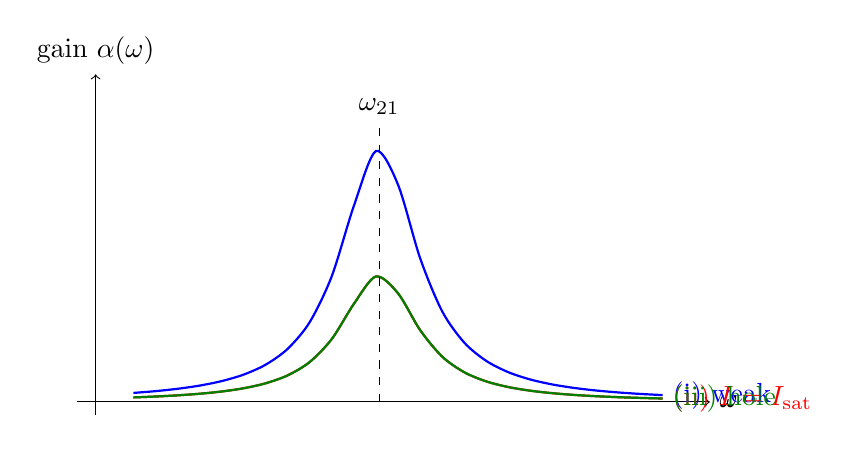
\begin{tikzpicture}[xscale=1.2,yscale=1.6]
\draw[->] (-0.2,0)--(6.5,0) node[right]{$\omega$};
\draw[->] (0,-0.1)--(0,2.6) node[above]{gain $\alpha(\omega)$};
\draw[domain=0.4:6.0,smooth,thick,blue] plot (\x,{2.0/(1+(\x-3)^2*4)}) node[right,blue]{(i) weak};
\draw[domain=0.4:6.0,smooth,thick,red] plot (\x,{1.0/(1+(\x-3)^2*4)}) node[right,red]{(ii) $I=I_{\mathrm{sat}}$};
\draw[domain=0.4:6.0,smooth,thick,green!50!black] plot (\x,{2.0/(1+(\x-3)^2*4) - 1.0/(1+(\x-3)^2*4)}) node[right,green!50!black]{(iii) hole};
\draw[dashed] (3,0)--(3,2.2) node[above]{$\omega_{21}$};
\end{tikzpicture}
\end{center}

(i) A weak beam sees the unsaturated Lorentzian $\alpha_{0}/[1+(\omega-\omega_{21})^{2}/(\Delta\omega_{H}/2)^{2}]$ of peak height $\alpha_{0}$ and FWHM $\Delta\omega_{H}$.

(ii) A beam of intensity $I=I_{\mathrm{sat}}$ saturates the medium: the gain is reduced everywhere, with the deepest reduction at line centre. From \eqref{eq:gain-sat} it is straightforward to show that the saturated profile is itself Lorentzian, with reduced peak $\alpha_{0}/2$ and \emph{broadened} FWHM $\sqrt{2}\Delta\omega_{H}$ --- this is power broadening.

(iii) When the medium is irradiated by a strong saturating beam at frequency $\omega_{21}$ and the gain is probed by an independent \emph{weak} beam at variable $\omega$, the two beams interact with the \emph{same} atomic class (the medium is homogeneously broadened, so every atom contributes to every frequency). The strong beam therefore reduces $N^{*}$ uniformly across the line and the weak probe sees the same saturated curve as in (ii). The strict statement is: in a homogeneously broadened medium all atoms contribute coherently, so a saturating beam at $\omega_{21}$ saturates the gain at \emph{every} frequency (no spectral hole burned). Thus case (iii) coincides with case (ii) for a homogeneously broadened transition; the two would differ only for an inhomogeneously broadened medium, where (iii) would burn a spectral hole. The figure above sketches the homogeneous result.

\subsection*{(d) Two broadening mechanisms in the He--Ne laser at 633\,nm}

The dominant broadening of the Ne $3\mathrm{s}_{2}\to 2\mathrm{p}_{4}$ laser transition at $\lambda=\SI{633}{nm}$ is \emph{Doppler broadening} (the gas is at $T\sim \SI{400}{K}$ and pressures are low, so collisions are rare). This is the inhomogeneous mechanism: each atom emits at a frequency Doppler-shifted by its longitudinal velocity. The Doppler FWHM is
\begin{equation}
\Delta\nu_{D} = \frac{2}{\lambda}\sqrt{\frac{2k_{B}T\ln 2}{m}}.
\label{eq:Doppler}
\end{equation}
The full envelope of the gain curves in the figure is $\sim \SI{500}{MHz}$, consistent with $\Delta\nu_{D}\simeq \SI{1.5}{GHz}$ for $T\sim \SI{400}{K}$ (the figure shows roughly half of this band; in practice the gain extends to either side of the cavity-free-spectral-range plotted). Solving \eqref{eq:Doppler} for $T$ with $\Delta\nu_{D}=\SI{1.5}{GHz}$, $\lambda=\SI{633}{nm}$, $m=\SI{20}{u}=\SI{3.32e-26}{kg}$:
\[
T=\frac{m c^{2}}{8 k_{B}\ln 2}\!\left(\frac{\Delta\nu_{D}}{\nu}\right)^{2}\simeq \SI{400}{K},
\]
a sensible discharge-tube temperature.

The homogeneous mechanism is \emph{natural (lifetime) broadening} together with \emph{pressure (collisional) broadening}. The natural width of the Ne 633\,nm upper level is $\Delta\nu_{N}=A_{21}/(2\pi)\sim \SI{10}{MHz}$ (the $3\mathrm{s}_{2}$ level has a radiative lifetime $\sim \SI{30}{ns}$, dominated by other decay channels; the partial $A_{21}$ for the 633\,nm line itself is smaller). At HeNe gas pressures $\sim 1\,$mbar the pressure broadening is comparable, $\sim \SI{10}{MHz}$. Combining the two homogeneous contributions in quadrature for a Lorentzian gives a homogeneous FWHM around $\SI{20}{MHz}$, in good agreement with the $\SI{30}{MHz}$ Lamb-dip width quoted for curve $A$ (see (e) below). The relevant physical estimate is therefore
\begin{equation}
\boxed{\;\Delta\nu_{H}\sim \frac{1}{2\pi\tau_{2}}+\frac{1}{2\pi\tau_{1}}+\frac{n\sigma_{\mathrm{coll}}\bar v}{2\pi}\sim \SI{20}{MHz},\;}
\label{eq:Lorentz-FWHM}
\end{equation}
where $\tau_{1,2}$ are the lower- and upper-level lifetimes; $n$ is the gas density; $\sigma_{\mathrm{coll}}\sim \SI{e-19}{m^{2}}$ is the collisional cross-section; $\bar v\sim \SI{700}{m\,s^{-1}}$ is the mean thermal speed. With $\tau_{2}\sim 30\,$ns, $\tau_{1}\sim 10\,$ns, and pressure $\sim 1$\,mbar one indeed obtains tens of MHz.

\subsection*{(e) Why a Lamb dip appears, and why it broadens with $R_{2}$}

\paragraph{Mechanism.} The HeNe gain is \emph{inhomogeneously} broadened (Doppler), so the laser cavity standing wave at frequency $\omega$ interacts with two distinct velocity classes: atoms with longitudinal velocity $v_{z}$ such that $\omega(1-v_{z}/c)=\omega_{21}$ (driven by the ``forward'' running wave) and $v_{z}\to -v_{z}$ (the ``backward'' running wave). At $\omega \neq \omega_{21}$ these two classes are different atoms, so the saturating effect of each running wave on the other is small; the gain is large. \emph{Exactly at} $\omega=\omega_{21}$ the two velocity classes coincide ($v_{z}=0$), so each running wave saturates the same atoms as the other. The total saturation rate is doubled and the gain is reduced --- the Lamb dip. The width of the dip is the homogeneous width $\Delta\nu_{H}$ of \eqref{eq:Lorentz-FWHM}, since only $|v_{z}|<c\Delta\nu_{H}/\nu$ is saturated by either wave on its own.

\paragraph{Broadening with $R_{2}$.} As the discharge current (and hence $R_{2}$) increases, the intracavity intensity inside the cavity grows. From the discussion in (c), a saturating beam at the line centre power-broadens the homogeneous Lorentzian profile from FWHM $\Delta\nu_{H}$ to $\Delta\nu_{H}\sqrt{1+I/I_{\mathrm{sat}}}$. For curve A the fractional saturation must be small ($I/I_{\mathrm{sat}}\sim 1$ gives a $\sqrt{2}$ broadening, consistent with the ratio $\SI{40}{MHz}/\SI{30}{MHz}\simeq 1.33$). Therefore
\begin{equation}
\boxed{\;\Delta\nu_{\mathrm{dip}}=\Delta\nu_{H}\sqrt{1+I/I_{\mathrm{sat}}}\;}
\label{eq:dip-broadening}
\end{equation}
and the broadening from $30\to 40$\,MHz between curves $A$ and $C$ is consistent with $I/I_{\mathrm{sat}}\simeq (40/30)^{2}-1\simeq 0.78$. Physically, increasing the discharge current pumps more atoms into the upper laser level, raising the intracavity field above threshold and thereby \emph{power broadens} the spectral hole that the standing wave burns at $v_{z}=0$. (Other effects --- collisional broadening at higher current --- also contribute, but power broadening is the dominant mechanism.)

\end{document}
